%% \typeout{IJCAI--22 Instructions for Authors}

% These are the instructions for authors for IJCAI-22.

\documentclass{article}
\pdfpagewidth=8.5in
\pdfpageheight=11in
% The file ijcai22.sty is NOT the same as previous years'
\usepackage{ijcai22}

% Use the postscript times font!
\usepackage{times}
\usepackage{soul}
\usepackage{url}
\usepackage[hidelinks]{hyperref}
\usepackage[utf8]{inputenc}
\usepackage[small]{caption}
\usepackage{graphicx}
\usepackage{amsmath}
\usepackage{amsthm}
\usepackage{booktabs}
\usepackage{algorithm}
\usepackage{algorithmic}
\usepackage{multirow}
\urlstyle{same}

% the following package is optional:
%\usepackage{latexsym}

% See https://www.overleaf.com/learn/latex/theorems_and_proofs
% for a nice explanation of how to define new theorems, but keep
% in mind that the amsthm package is already included in this
% template and that you must *not* alter the styling.
% \newtheorem{example}{Example}
% \newtheorem{theorem}{Theorem}

% Following comment is from ijcai97-submit.tex:
% The preparation of these files was supported by Schlumberger Palo Alto
% Research, AT\&T Bell Laboratories, and Morgan Kaufmann Publishers.
% Shirley Jowell, of Morgan Kaufmann Publishers, and Peter F.
% Patel-Schneider, of AT\&T Bell Laboratories collaborated on their
% preparation.

% These instructions can be modified and used in other conferences as long
% as credit to the authors and supporting agencies is retained, this notice
% is not changed, and further modification or reuse is not restricted.
% Neither Shirley Jowell nor Peter F. Patel-Schneider can be listed as
% contacts for providing assistance without their prior permission.

% To use for other conferences, change references to files and the
% conference appropriate and use other authors, contacts, publishers, and
% organizations.
% Also change the deadline and address for returning papers and the length and
% page charge instructions.
% Put where the files are available in the appropriate places.

% PDF Info Is REQUIRED.
% Please **do not** include Title and Author information
\pdfinfo{
  /TemplateVersion (IJCAI.2022.0)
}

\title{IJCAI--22 Formatting Instructions}

% Single author syntax
%% \author{
%%     Author Name
%%     \affiliations
%%     Affiliation
%%     \emails
%%     pcchair@ijcai-22.org
%% }

% Multiple author syntax (remove the single-author syntax above and the \iffalse ... \fi here)

\author{
  Arumoy Shome$^1$
  \and
  Lu{\'\i}s Cruz$^1$\And
  Arie van Deursen$^{1}$
  \affiliations
  $^1$Delft University of Technology\\
  \emails
  \{a.shome, l.cruz, arie.vandeursen\}@tudelft.nl
}


\begin{document}

\maketitle

\begin{abstract}
  %% TODO
  This is an abstract that I am writing \cite{sambasivan}.
\end{abstract}

\appendix

\section{Introduction}\label{sec:intro}
%% TODO

%% present a general motivation of the problem space & the problem we
%% are trying to solve

%% present research questions that we want to answer along with brief
%% preview of results

%% RQ1: can we minimise fairness testing by only testing the data?
%% RQ2: can we minimise to data fairness testing when experimenting
%% with training size?
%% RQ3: can we minimise to data fairness metrics when experimenting
%% with feature size?

\section{Background \& Related Work}\label{sec:related}
%% TODO

%% summarise the current work on fairness testing; touch upon this
%% aspect from a SE perspective; the fairness metrics we have (and why
%% we use specific ones);
\begin{table}[htb]
  \centering
  \caption{Datasets used in the study}
  \begin{tabular}{p{0.3\linewidth} p{0.1\linewidth} p{0.1\linewidth} r r r}
    \toprule

    \textbf{Name} & \textbf{Protected} & \textbf{Abbr.} &
    \textbf{Total} & \textbf{Positive} & \textbf{Negative}\\

    \midrule

    \multirow{2}{*}{Adult Income \cite{CITEME}} & sex & adult-sex & 45222 & 11208 &
    34014\\
      & race & adult-race & 45222 & 11208 & 34014\\
    \multirow{2}{*}{Compas Score \cite{CITEME}} & sex & compas-sex &
    6167 & 3358 & 2809\\
      & race & compas-race & 6167 & 3358 & 2809\\
    Bank Marketing \cite{CITEME} & age & bank-age & 30488 & 3859 &
    26629\\
    \multirow{2}{*}{German Credit \cite{CITEME}} & sex & german-sex &
    1000 & 700 & 300\\
      & age & german-age & 1000 & 700 & 300\\
    Medical Survey 2021 \cite{CITEME} & race & meps-race & 15675 &
    2628 & 13047\\
    \bottomrule
  \end{tabular}
  \label{tab:datasets}
\end{table}
%% TODO brief commentary on tab:datasets, the ones we use (and why),
%% the range of examples; short comment on pre-existing bias in the
%% dataset.

%% list the fairness metrics we use in our analysis & why


\begin{equation}
  DI_{data} = \frac{P(Y=1|D=0)}{P(Y=1|D=1)}
  \label{eq:di-data}
\end{equation}

\begin{equation}
  DI_{model} = \frac{P(\hat{Y}=1|D=0)}{P(\hat{Y}=1|D=1)}
  \label{eq:di-model}
\end{equation}

\begin{equation}
  SPD_{data} = P(Y=1|D=0)-P(Y=1|D=1)
  \label{eq:spd-data}
\end{equation}

\begin{equation}
  DI_{model} = P(\hat{Y}=1|D=0)-P(\hat{Y}=1|D=1)
  \label{eq:spd-model}
\end{equation}

%% list the ML models we use in our analysis and why (because we want
%% to generalise over multiple datasets)

\section{Methodology}\label{sec:method}
%% TODO should we include numbers conditioned on
%% privileged/unprivileged?

%% - we use 5 popular datasets from the fairness literature
%% - we use 4 popular ML models used in prior fairness testing
%% literature
%% - we use 2 popular group fairness metrics used in the fairness
%% literature
%% - we calculate fairness metrics first on the data (DFM) and next on
%% the predictions of the model on the test set (MFM) and analyse the
%% results
%% - we normalise all results following the procedure used by
%% zhang2021ignorance 
%% - we use correlation & linear regression to analyse the
%% relationship between DFM & MFM; we observe that they are related to
%% one another; DFM can indicate fairness issues in the model with
%% statistical significance

%% outline the data collection setup; break this down by the
%% experiments (we have two); explain the slicing mechanism in each
%% experiment, how & why we are shuffling the example & feature orders

%% TODO definitely need to diagram; hard to explain experimental
%% design using only words

%% we only consider one protected attribute at a time; for feature
%% sets experiment, we consider a minimum of 3 features (in addition
%% to the protected attribute & target features)
Figure \ref{fig:exp-design} presents the experimental design for the
study. For each dataset, protected attribute and model tuple, we use a
75-25 split to create the training and test sets. There are two
flavours of fairness metrics calculated next. We calculate the DFMs on
the training set and the MFMs on the predictions of the model on the
test set. Next we analyse the DFM and MFM by observing the correlation
between them and by fitting a linear regression model. We repeat this
procedure 50 times and use statistical hypothesis testing to validate
that our results are statistically significant.

We extend the above experiment further in two ways (by adopting the
experimental design from \cite{zhang2021ignorance}). First, we
experiment with different number of training examples and second with
different number of features in the training set. For both examples,
we shuffle the order of the examples in the training and test sets. For
the feature sets experiment, we additionally shuffle the order of the
features.

For the training sets experiment, we create different sub-subsets of
the training subset from 10\% to 100\%. For the feature sets
experiment, we consider a minimum of 3 features (in addition to the
protected attribute and the target feature) to all features.

% TODO mention that we check the statistical significance of the
% correlation & linear regression analysis by observing the p values
% at 3 alpha levels: 0.01, 0.05 & 0.01

\section{Results \& Discussion}\label{sec:results}

%% as disclaimer: mention that for visual aids we typically focus on
%% the adult-sex dataset but results for all datasets is provided as
%% part of the replication package.

%% start with the smallest unit: full training data, show that there
%% is a positive correlation between the DFM & MFM for all models &
%% datasets. Show that linear regression is also positive.

%% move on to experiment with the training sets; use
%% zhang2021ignorance to show that most of the changes are
%% significant; show the correlation & linear regression results

%% finally present the feature sets experiment; again same
%% presentation order as training sets experiment.

%% list & explain the two tests we use to evaluate relationship
%% between data & model metrics (we have two: correlation & linear
%% regression)

%% present the results from the two experiments & our analysis

%% exp-training-sets: emphasise the importance of data quality. If we
%% look at the underlying data, the we need to link the results & our
%% discussion to the research questions we are trying to answer

\subsubsection{Full Training Set}\label{sec:results-full-data}

Figure \ref{fig:boxplot-di-spd-full} presents the distribution of the
%% or "we observe that DFM and MFM convey the same information..."
fairness metrics across the datasets. We observe that the DFM agree
with the MFM in all cases. SPD is observed to be more sensitive to the
size of the training set since the variability is higher in datasets
with lesser number of training examples. The variability of the DFM is
lesser compared to the MFM. This is because in addition to the
randomness from the data shuffling in the training set, the models are
assigned random initial states in every iteration. Finally, the tree
based classifiers (DT and RF) make fairer decisions compared to the
other classifiers, sometimes even better than the baseline provided by
the DFM.

%% TODO investigate large variability in the bank-age dataset.
%% 2022-12-05 I have some a possible explaination, but not sure if it
% is the right one

\begin{figure}
  \centering
  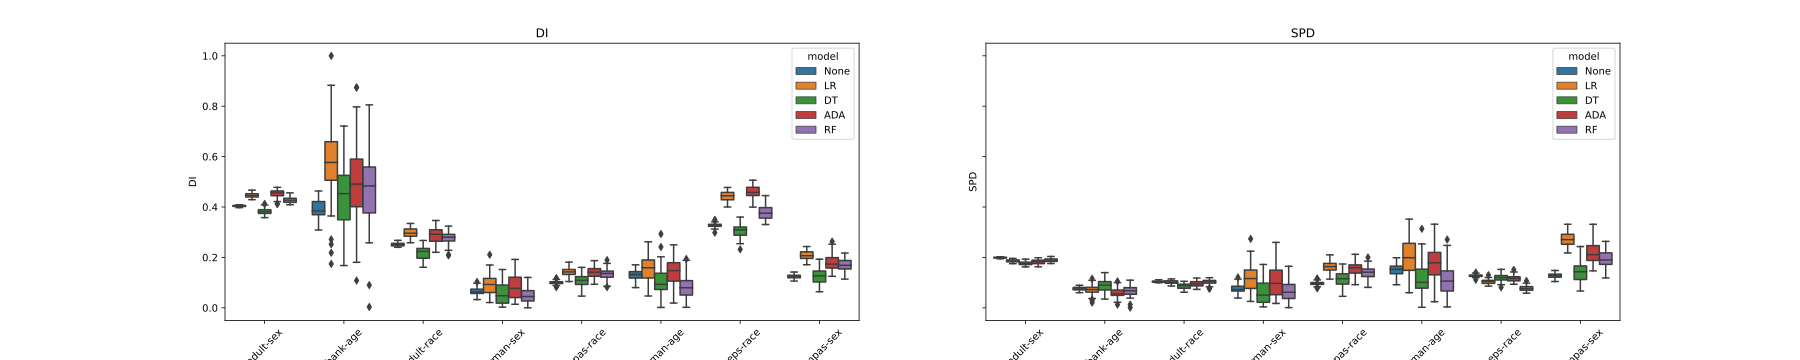
\includegraphics[width=0.95\linewidth]{boxplot--dataset--di-spd--exp-full.pdf}
  \caption{Distribution of DFM and MFM across datasets}
  \label{fig:boxplot-di-spd-full}
\end{figure}

Figure \ref{fig:heatmap-corr-full-data} shows the correlation between
the DFM and the MFM across all models and datasets. We primarily
observe darker colors in the heatmap indicating that there is no
significant correlation between the DFM and MFM in most of the
cases. As noted in the distribution analysis above, we see less
variability in DFM compared to MFM. In the correlation analysis we are
therefore trying to explain the additional variability in the MFM
using the limited variability in the DFM, which is not possible.

\begin{figure}
  \centering
  \includegraphics[width=0.95\linewidth]{heatmap--corr--full-data.pdf}
  \caption{Correlation between DFM and MFM}
  \label{fig:heatmap-corr-full-data}
\end{figure}

We observe 14 cases however, where the correlation is statistically
significant. For these cases, we additionally conduct linear
regression analysis. Figure \ref{fig:scatterplot-dfm-mfm-adult-race}
and \ref{fig:scatterplot-dfm-mfm-compas-race} represent two
contrasting examples. Figure \ref{fig:scatterplot-dfm-mfm-adult-race}
presents the linear regression fit along with the scatter plot of the
residuals for the \emph{adult-race} dataset and decision tree model.

%% TODO commentary on linear regression + residual plots

\begin{figure}
  \centering
  \includegraphics[width=0.95\linewidth]{scatterplot--dfm--mfm--adult-race.pdf}
  \caption{Correlation between DFM and MFM}
  \label{fig:scatterplot-dfm-mfm-adult-race}
\end{figure}

\begin{figure}
  \centering
  \includegraphics[width=0.95\linewidth]{scatterplot--dfm--mfm--compas-race.pdf}
  \caption{Correlation between DFM and MFM}
  \label{fig:scatterplot-dfm-mfm-compas-race}
\end{figure}

%% move to the correlation analysis from here; explain why we primarily
%% have no correlation; comment on the few examples where we do have a
%% strong (positive or negative) correlation & that they are
%% statistically significant; in our analysis we recommend that if its
%% possible in some cases then we should always test for fairness;
%% comment on the meaning behind the direction of the correlation; no
%% correlation means that we need both for testing; positive means
%% there is a possibility for prioritisation; interpretation of
%% negative correlation is bit more challenging; use a lineplot to
%% show that the DFM does not change as much, for the cases where we
%% have a negative correlation, show that the MFM decreased (meaning
%% the model learned to make fair predictions) and the cases where
%% there was a positive correlation the model simply
%% reflected/amplified the bias in the data

\subsubsection{Training Sets Experiment}

\subsubsection{Feature Sets Experiment}

\section{Threats to Validity}\label{sec:threats}
%% TODO we did not look at the underlying distribution of the training
%% dataset (which is biased to begin with); it will be interesting to
%% evaluate if we can minimize fairness testing when we utilise bias
%% mitigation techniques

% note on linear regression model: we used ordinary-least squares with
% degree 1 to estimate the fit; we tried different degrees with
% model=DT and dataset=adult-sex; we also investigated baysian linear
% regression

% pvalue for scipy.stats.spearmanr is not reliable for datasets less
% than 500 examples; this is a threat for the full-data experiment
% since we only have 50 observations per model-dataset combo; this
% means that with more iterations we may see a correlation with
% significance where currently there is none; but this does not change
% our final recommendation which is to test with both data & model in
% these cases

\section{Conclusion}\label{sec:conclude}
%% TODO

\bibliographystyle{named}
\bibliography{report}

\end{document}

